\documentclass{article}
\fonts{dir="../../corpus/fonts",body="Source Serif Pro",math="Fira Math"}
\usepackage{tikz}
\usepackage{amsmath}
\usepackage[makeroom]{cancel}
\pictures{tool=none}
\title{A route through four stations}
\author{}
\date{}
\begin{document}
\maketitle

This note describes a fictional route for wooden tokens. A prime marks a
revised station, and a subscript marks a reserve station. The lower labels
record a ratio and a root used when sorting the tokens.

\begin{center}
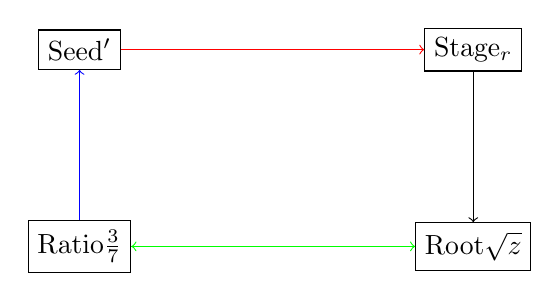
\begin{tikzpicture}
\node[draw,rectangle] (seed) at (0,0) {Seed$'$};
\node[draw,rectangle] (stage) at (5,0) {Stage$_r$};
\node[draw,rectangle] (ratio) at (0,-2.5) {Ratio$\frac{3}{7}$};
\node[draw,rectangle] (root) at (5,-2.5) {Root$\sqrt{z}$};
\draw[->,red] (seed) -- (stage);
\draw[->,blue] (ratio) -- (seed);
\draw[->,green] (ratio) -- (root);
\draw[->,green] (root) -- (ratio);
\draw[->,black] (stage) -- (root);
\end{tikzpicture}
\end{center}

The red route goes right, the blue route returns upward, the green route
works in both directions, and the black route goes down. Each arrow ends
at a station boundary so that its label remains readable.

\section{A sample reduction}
The trial contribution is discarded while the neighboring terms remain.
Its target is a zero weight, written with the unit variable \(g\).
\[
u+\cancelto{0g}{\frac{x}{\sqrt{y}}}+v
\]
The route and the reduction describe separate steps of the same toy process.
\end{document}
